\documentclass[usletter]{article}
\usepackage{graphicx}
\usepackage{amsfonts}
\usepackage{amsthm}
\usepackage{amsmath}
\usepackage{amssymb}
\usepackage{scribe}
\usepackage[margin=1.5in]{geometry}

\begin{document}

\makeheader{Lowell Bander}{January 4, 2016}{1}{Deterministic Computation}

\noindent
During the first lecture of the course, we covered the formalisms for and semantics of the \emph{Turing Machine} (TM), a universal model of computation. We then proceeded to describe a TM which checks whether its input is a palindrome, so as to demonstrate how to construct a TM to solve an arbitrary problem.

During the second half of the lecture, we covered the notion of efficiency as it pertains to the time a TM takes to compute its output. Lastly, we showed that our standard definition of a TM can be used to simulate more complicated TM's, such as those with an enriched alphabet and those with bidirectional tapes. This last bit comes back to the notion that the Turing Machine is in fact a universal model of computation -- it can compute anything which is computable, even things which may seem to be computable only with more complex models of computation.

\section{Turing Machines Defined}
\label{sec:tmdef}

As mentioned in the preceding paragraphs, a Turing Machine (TM) is a universal model of computation. That is, it can simulate any computer algorithm, but this is not to say that it wouldn't be cumbersome to do so. For example, computing the first several numbers of the Fibonacci Sequence or creating an operating system would be much more easily done with languages such as Python and C, respectively, but both computations can be simulated with a TM. 

\begin{figure}[h!]
\begin{center}
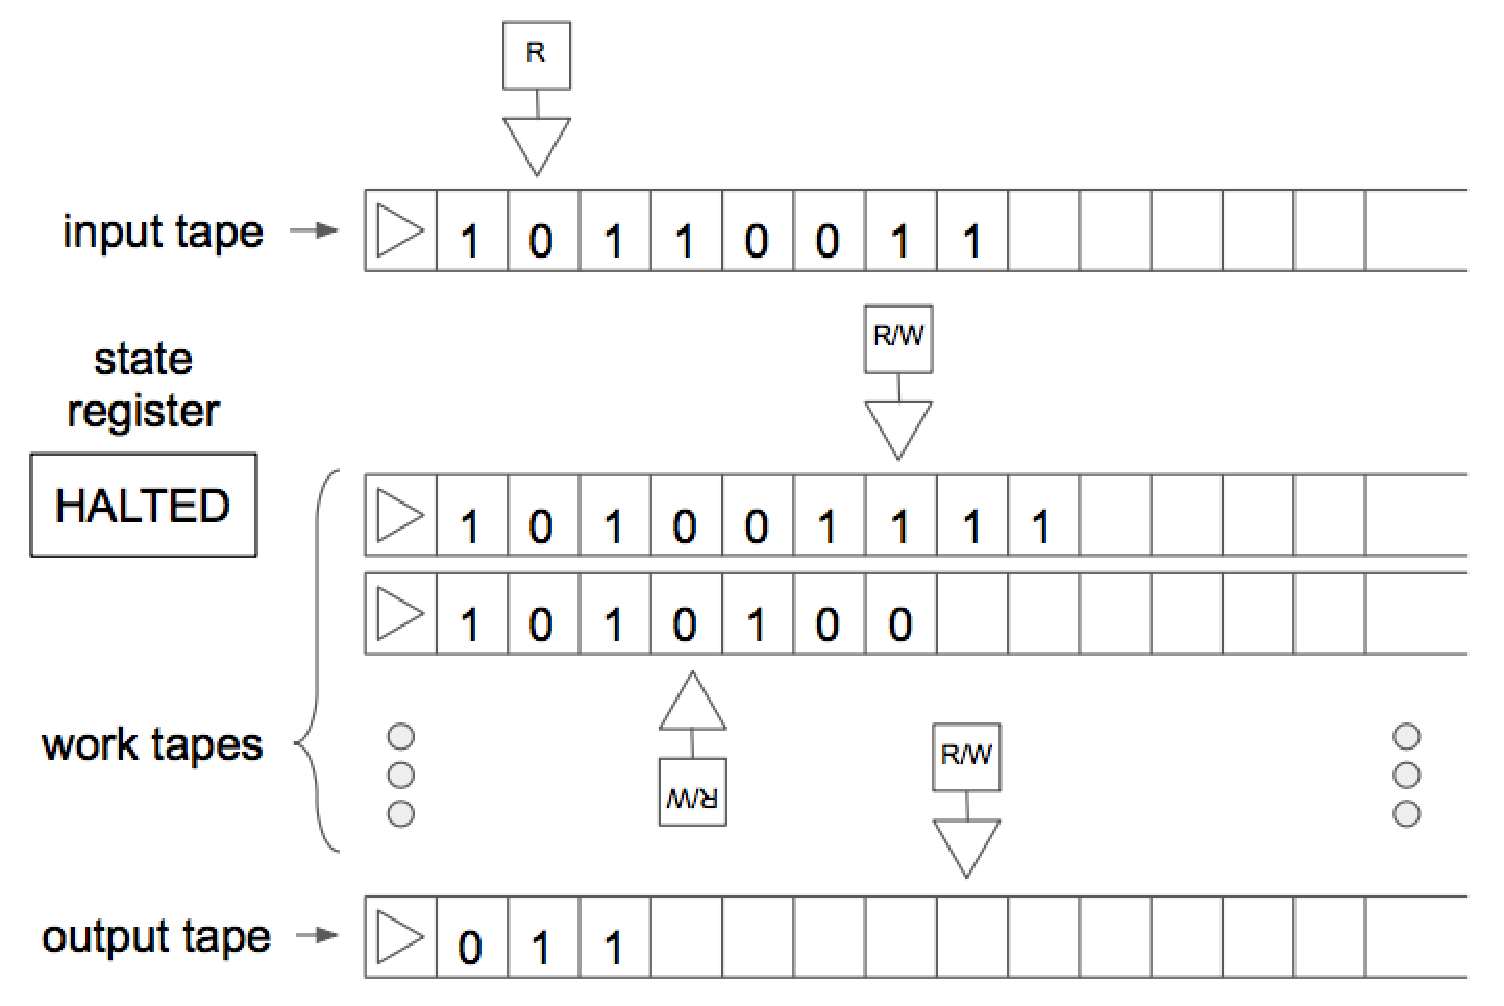
\includegraphics[width=\textwidth]{tm}
\end{center}
\caption{A standard Turing Machine.}
\label{fig:tm}
\end{figure}

As can be seen in Figure~\ref{fig:tm}, a TM consists of arbitrarily many tapes whose cells are capable of storing values. The first tape is known as the \emph{input tape}, and is used to represent the input to the TM, as its name suggests. The final tape in the TM is known as the \emph{output tape} and stores the result of the computation done by the TM. The remaining tapes are known as \emph{work tapes} and are used as a sort of scratch pad for the intermediate computation done by the TM.

The entities floating about the tapes in Figure~\ref{fig:tm} are \emph{tape heads}, all of which (except for the head of the input tape, which can only read) are capable of reading values from and writing values to the segment of the tape which they are pointing to at a given point in time. Additionally, all tape heads can either move to the left, move to the right, or stay put at each step in the computation performed by the TM.

Lastly, a TM has a a state register which is capable of storing, at any given time, one of the finitely many states available to the TM. In Figure~\ref{fig:tm}, the state register holds the value $HALTED$, which is the state a TM enters once it has finished computation.

Figure~\ref{fig:tm} and the accompanying description provides a useful visual intuition for the composition and behavior of a TM. However, it often proves useful to refer to the mathematical formalism of a TM, which is as follows. Formally, a TM is a tuple $(\Gamma, Q, \delta)$, such that $\Gamma$ is the alphabet of the TM, a finite set of symbols which has at minimum the subset $\{\Box, \rhd, 0, 1\}$, where $\Box$ is used for blank segments on the TM's tapes, and the $\rhd$ denotes the leftmost segment of a tape; $Q$ is a set of states which at minimum contains the states $START$ and $HALTED$, which are used, respectively, for the initial and final states of computation; and lastly $\delta$, the \emph{transition function} for the TM, which is used to determine what state to enter, what symbols to write to the tapes, and which direction (if any) to move each head, all based on the current state and the symbols beneath the every head of the TM. The transition function $\delta$ thus takes the following form: 

\begin{align}
\delta : Q \times \Gamma^k \rightarrow Q \times \Gamma^{k-1}\times \{\leftarrow, \cdot, \rightarrow\}^k
\end{align}
where $k$ is the number of total tapes in the TM. The superscript for $\Gamma$ in the domain and for the set $\{\leftarrow, \cdot, \rightarrow\}$ in the codomain is $k$ because all $k$ tapes are examined when determining the behavior of the TM in the current step, and all $k$ tapes can either move or stay put in any given step. Similarly, the superscript for $\Gamma$ in the codomain of $\delta$ is $k-1$ because all tapes have new values written to the segment currently pointed to by their respective heads except for the input tape, because its head is read-only.

Though the semantics of the TM have been hinted at in the description above, they are included here explicitly for good measure. At the start of computation, the TM is in the $START$ state, the input tape contains the input to the TM, all heads are at the leftmost positions of their respective tapes, and all tapes contain only $\Box$, save for the leftmost cell of each tape which contains a $\rhd$. Then, during each step of computation, based on the symbols observed by the heads and on the current state, the TM will write new symbols to the cells pointed to by the tape heads (sans the input tape), and then move the tape heads according to $\delta$. Computation ultimately completes once the TM enters the $HALTED$ state.

\section{Example Turing Machine: Palindrome Checker}

Having discussed the structure and function of a TM, we now demonstrate how to describe a TM to solve a particular problem. For no particular reason, we have chosen to create a TM which checks whether its input is a palindrome, that is, whether the input looks the same when read forwards as it does when read backwards.

\begin{definition}
A string $x \in \{0,1\}^n$ is a palindrome iff $x_1x_2...x_n = x_n...x_2x_1$.
\end{definition}
\noindent
For example, the strings 10101, 0, 11, and 000 are all palindromes, but the strings 10,  011, and 10111 are not.

One way to create a palindrome checker using a TM is as follows.
\begin{itemize}
\item The TM will have 3 tapes: an input tape, a single work tape, and an output tape.
\item $\Gamma = \{\Box, \rhd, 0, 1\}$
\item $Q = \{START, COPY, LEFT, TEST, HALTED\}$
\end{itemize}

The TM, like all TM's, starts in the $START$ state. Then, while in the $COPY$ state, the TM copies the contents of the input tape to the work tape. The TM then enters the $LEFT$ state, during which the input tape's head moves to the left-most position. Then, during the $TEST$ state, the heads of the input and work tape check to see if the cells they point to contain the same value; if they do, the head of the input tape moves right, and the head of the work tape moves left; if the values are not the same, a 0 is written to the output tape and the $HALTED$ state is entered. If the $HALTED$ state is not entered by the time the head of the work tape reaches the left-most position, then the input string is a palindrome, and so a 1 is written to the output tape and the TM enters the $HALTED$ state.

It should be noted that is by no means the only manner in which to implement a TM which checks whether its input is a palindrome. For example, such a TM could have been implemented without a work tape, and instead the head of the input tape would zig and zag across the input tape to check to see if the first and last symbols matched, if the second and second to last symbols matched, and so on. This new implementation uses less space but more time than our initial solution, which brings us to our next topic.

\section{Efficiency}

We now introduce the notion of efficiency, and the formalism with which we will quantify the performance of an arbitrary TM. First, we let $f : \{0,1\}^* \rightarrow \{0,1\}^*$ be our function of interest, and $T : \mathbf{N} \rightarrow \mathbf{N}$ be a time bound.

\begin{definition}
Turing Machine $M$ computes $f$ in time $T(n)$ if, when started with $x \in \{0,1\}^*$ written on the input tape, halts within time $T(|x|)$ with $f(x)$ written on the output tape.
\end{definition}

The bars surrounding the input string denote the bit length of the string. For example, $|10101| = 5$.

We now have the means with which to quantify the time-performance of the first palindrome checking TM we constructed. Namely, it has completes in time $3\cdot T(n) = O(n)$. Moreover, we can combine our newly produced definition of time efficiency with some definitions of what it means to be a language to define families of languages.

\begin{definition}
A language is any subset $L \subseteq \{0,1\}*$.
\end{definition}

That is to say, a language is any collection of binary strings.

\begin{definition}
Turing Machine $M$ \emph{decides} a language $L \subseteq \{0,1\}^*$ if $M$ computes the associated function $f_L : \{0,1\}^* \rightarrow \{0,1\}*$ where
\[f_L(x)= \begin{cases} 
      1 & \text{if } x \in L \\
      0 & \text{otherwise}
   \end{cases}
\]
\end{definition}

Using the preceding definitions, we can construct our first family of languages, $DTIME(T(n))$.

\begin{definition}
$DTIME(T(n))$ is the family of all languages $L$ decidable in time $c\cdot T(n)$ for some $c>0$.
\end{definition}

\begin{definition}
\begin{align}
P &= DTIME(n) \cup DTIME(n^2) \cup DTIME(n^3) \cup \dots\\
&= \bigcup\limits_{i=1}^{\infty} DTIME(n^i)
\end{align}
\end{definition}

That is, $P$ is the set of all languages which can be decided in polynomial time.

\section{Other Definitions of Turing Machines}

For this final section, we demonstrate that our standard TM as defined in Section~\ref{sec:tmdef} can simulate more complex TM's. In effect, this shows that although, for example, enriching the alphabet of a TM or makings its tapes bidirectional may make it more wieldy, that this does nothing to improve the expressive power of the standard TM.

First, we show that a TM with an enriched alphabet can be perfectly simulated by a standard TM, although it will do so more slowly.

\begin{definition}
If $f_L : \{0,1\}^* \rightarrow \{0,1\}^*$ is computable in time $T(n)$ with alphabet $\Gamma$, then $f$ is computable in time $O(T(n)\cdot \log_2|\Gamma|)$.
\end{definition}

Essentially, we accommodate this enriched alphabet within our restricted alphabet by encoding in binary every symbol in the enriched alphabet. For example, if the tapes of the TM with an enriched alphabet are as pictured in Figure??, we can use the encoding scheme in Table?? to generate a new set of tapes using only our restricted alphabet, as pictured in Figure??.

\begin{proof}
Encode each symbol of $\Gamma$ by a string in $\{0,1\}$* of $\log_2|\Gamma|$ bits.



\end{proof}

\end{document}
